\documentclass{sciposter}
\usepackage{epsfig}
\usepackage{amsmath}
\usepackage{amssymb}
\usepackage{multicol}

\usepackage{hyperref}
\usepackage{graphicx,url}
\usepackage[spanish, es-tabla]{babel}   
\usepackage[utf8]{inputenc}
%\usepackage{fancybullets}
\newtheorem{Def}{Definition}



\title{Caracterización de espectros de rayos X asociados a fuentes de tungsteno y plata usando un detector MEDIPIX3}
%Título do projeto

\author{López Juan, Barbosa Juan}
%nome dos autores

\institute 
{Departamento de Física\\
Universidad de los Andes\\
Cra 1 N$^\circ$ 18A - 12 Bogotá, Colombia}

\email{jc.lopez11@uniandes.edu.co, js.barbosa10@uniandes.edu.co}

%\rightlogo[1]{logo}
\leftlogo[2]{logo}


\begin{document}
\maketitle

%%% Begin of Multicols-Enviroment
\begin{multicols}{3}

%%% Abstract
\begin{abstract}
	El laboratorio de Altas Energías de la Universidad de los Andes cuenta con una fuente de rayos X de ánodo de tungsteno y en 2017 adquirió una fuente de rayos X de ánodo de plata. En este proyecto se presenta la caracterización de los espectros de dichas fuentes y su desempeño en la toma de imágenes usando un detector MEDIPIX3. Se observó que el espectro observado para las fuentes cambia su forma con el voltaje del tubo de rayos catódicos y que la fuente de rayos X de ánodo de plata produce un contraste más alto que el de la fuente de ánodo de tungsteno.
\end{abstract}

%%% Introduction
\section{Introducción}
\begin{itemize}
	\item Los ánodos determinan el espectro de emisión.
	\item El espectro depende de las transiciones electrónicas del ánodo.
	\item Las transiciones del tungsteno son de baja energía.
	\item La plata tiene trancisiones de más alta energía.
	\item Se desea tener espectros uniformes.
	\item Técnicas como XPS son sensibles al espectro de emisión.
\end{itemize}
%	\PARstart{L}{}os distintos tipos de ánodos presentes en las fuentes hacen que el espectro de emisión entre fuentes tengan una forma distinta. Puesto que la emisión de rayos X depende de la energía de las transiciones electrónicas del ánodo. En el caso del tungsteno, las transiciones se dan a más baja energía, presentando picos intensos en la parte más baja del espectro; mientras que en la plata se tienen transiciones más energéticas, de forma que se tienen picos de emisión más pequeños a más altas energías, dando lugar a una emisión más uniforme.
%	
%	Los efectos más notorios de la uniformidad del espectro son cambios en el tiempo de adquisición que se debe usar en los sensores \cite{range}. Aun más, para la toma de imágenes de tejidos se requiere operar en regiones del espectro con intensidad aproximadamente constante, con el fin de que sea posible observar las estructuras presentes con el mayor contraste posible. Lo que se busca, es que la diferencia en intensidades esté dada por la capacidad de absorción de las estructuras, en vez de estar dada por cambios en la intensidad de la fuente.
%	
%	En adición a esto, la existencia de energías preferenciales de emisión también ha de ser considerada en técnicas como XPS, en la cual se busca medir la composición elemental y tipos de enlace químico presentes en una muestra por medio de los picos de emisión de la misma, dado que los picos de emisión se muestran en el resultado final \cite{xps}. Siendo, entonces, necesario conocer detalladamente el espectro de emisión de la fuente para filtrar y obtener resultados correctos.

\section{Objetivos}
	Establecer diferencias en el funcionamiento de la fuente de rayos X de ánodo de Tungsteno y la fuente de rayos X de ánodo de Plata.
	\begin{enumerate}
		\item Probar el funcionamiento de la fuente de rayos X con ánodo de plata.
		
		\item Caracterizar la respuesta del sensor MEDIPIX3.
		
		\item Verificar el voltaje y la intensidad de cada fuente que produce la imagen con el mejor contraste.
		
		\item Hacer un estudio de cociente de señal a ruido de las diferentes imágenes obtenidas.
	\end{enumerate}

\section{Metodología}	
	\subsection{Tiempos de exposición}
	Los tiempos de exposición fueron seleccionados para maximizar conteos y evitar saturación.
	\begin{itemize}
		\item 2.5 s para la fuente de ánodo de tungsteno.
		\item Variable para la fuente de ánodo de plata. 
	\end{itemize}
	
	\begin{table}[h]
		\centering
		\small
		\begin{tabular}{| c | c c |}
			\hline
			\textbf{Voltaje (kV)} & \textbf{Corriente ($\mu$A)} & \textbf{Tiempo/TH (s)} \\
			\hline
			11.0 & 150.0 & 10.000 \\
			17.0 & 150.0 & 10.000 \\
			23.0 & 150.0 & 10.000 \\
			29.0 & 136.0 & 11.029 \\
			35.0 & 113.0 & 13.274 \\
			41.0 & 96.0 & 15.625 \\
			47.0 & 84.0 & 17.857 \\
			\hline
		\end{tabular}
		\label{tab:corrientes}
	\end{table}
	
	\subsubsection{\label{sec:medipix}Detector MEDIPIX3:}
	\begin{table}[h]
		\centering
		\small
		\begin{tabular}{| l | c |}
			\hline
			\textbf{Tipo} & \begin{tabular}[c]{@{}l@{}}MPX3RXV1, fine pitch\\ (55 $\mu$m pixel pitch)\end{tabular}  \\
			\textbf{Modo de operacion} & SPM \\
			\textbf{Preamp Gain} & High Gain Mode \\
			\textbf{No. serie} & W108-I4 \\
			\textbf{Polaridad del sensor} & N-on-P \\
			\textbf{Voltaje (V)} & -100V \\
			\hline
		\end{tabular}
		\label{tab:config_sensor}
	\end{table}
	
	\subsubsection{Barridos de voltaje y calibración de energía:}
	Se manufacturó una base móvil para la fuente de ánodo de plata.
	Se realizaron barridos de voltaje de 11 kV a 47 kV en pasos de 6 kV para las dos fuentes sin muestras. 
	
	\begin{figure}[h]
		\centering
		\begin{tabular}{cc}
			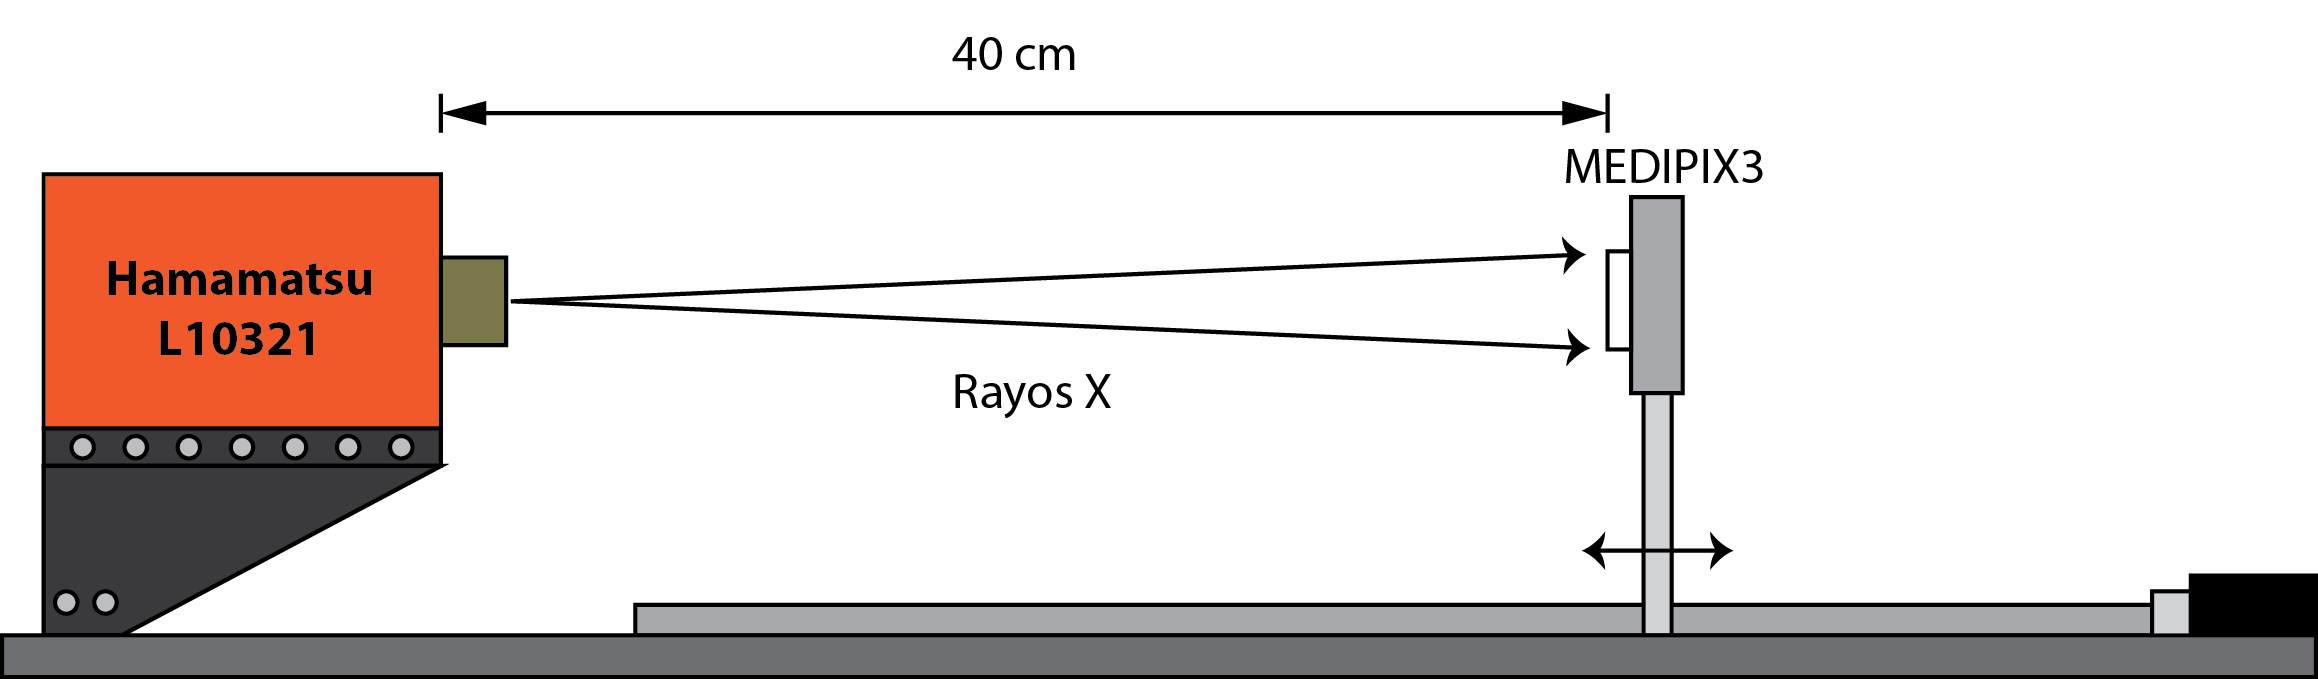
\includegraphics[width = 0.5\linewidth]{Figuras/W_Cal.png} & 
			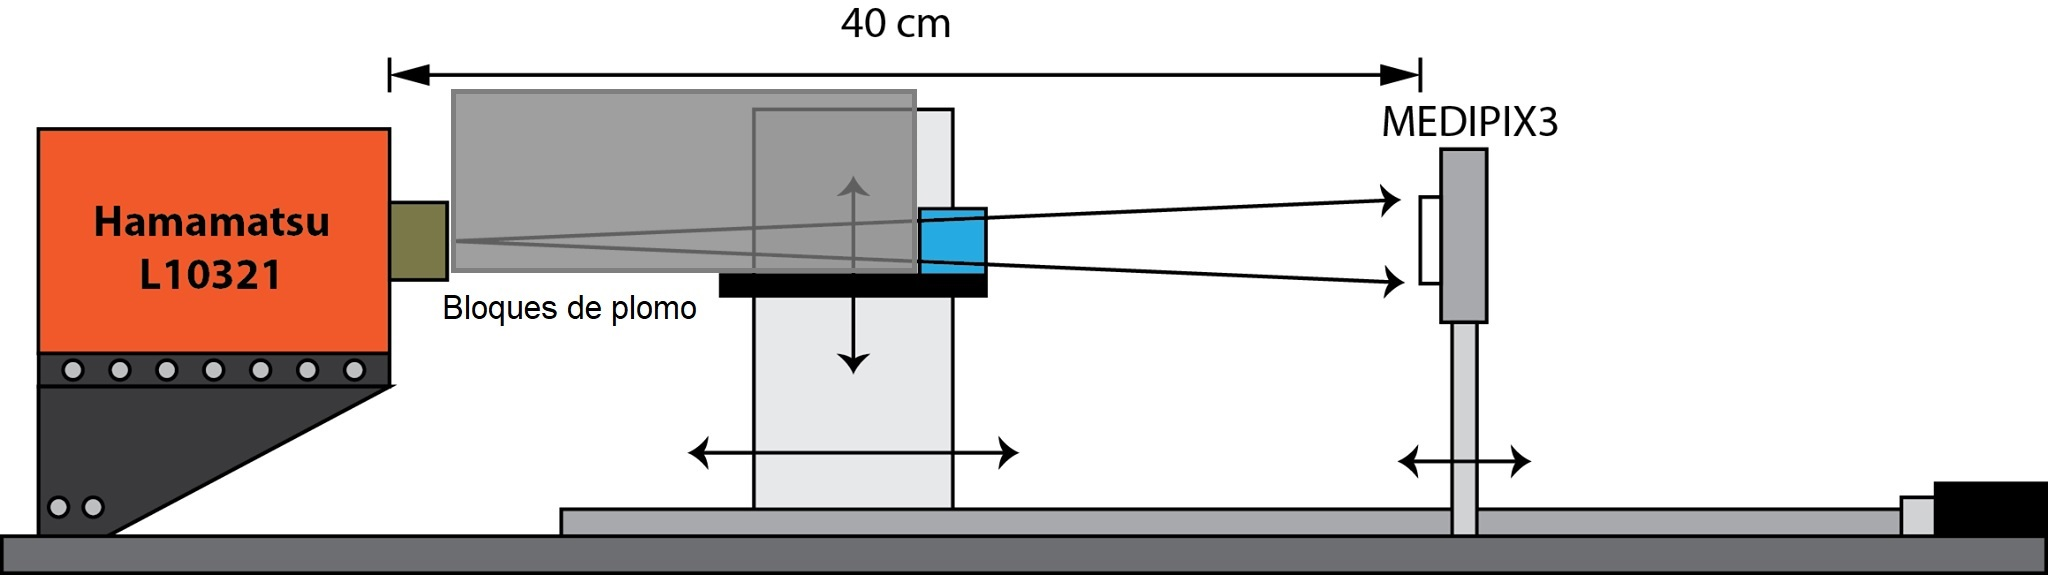
\includegraphics[width=0.5\linewidth]{Figuras/bloques.jpg}
		\end{tabular}
	\end{figure}
	
	\subsubsection{Relación señal a ruido:}
	Se calcula estadísticamente como:
	
	\begin{equation}
	SNR=\frac{\mu_{sig}}{\sigma_{sig}}
	\end{equation}
	
	\subsubsection{Toma de imágenes:}
	Muestra de acrílico con incrustaciones de calcita en el camino de los rayos X.
	Se toman todas las imágenes con la misma corriente de tubo.
	
	\begin{figure}[h]
		\centering
		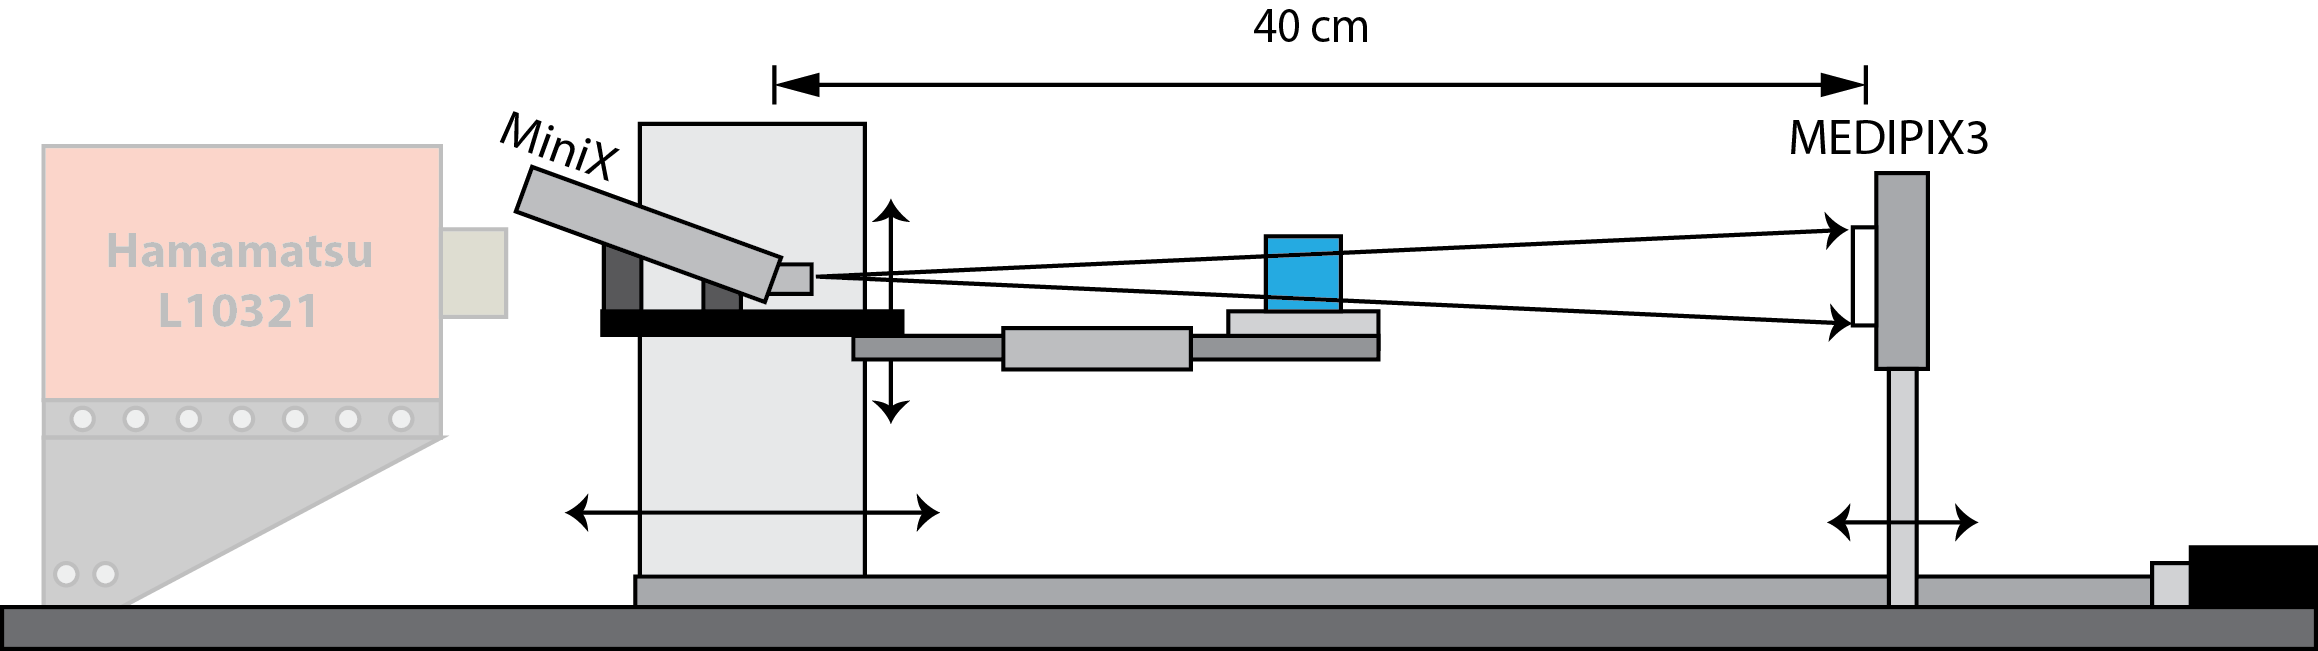
\includegraphics[width = 0.7\linewidth]{Figuras/Ag_Ima.png}
	\end{figure}

\section{Resultados y discusión}
	Se estableció la equivalencia entre DAC y eV con espectros de rodio y cobre.
	
	\begin{equation}
	[\frac{DAC}{eV}]=\frac{DAC_{Rh}-DAC{Cu}}{K\alpha_{Rh}-K\alpha_{Cu}}
	\end{equation}
	
	\begin{figure}[h]
		\centering
		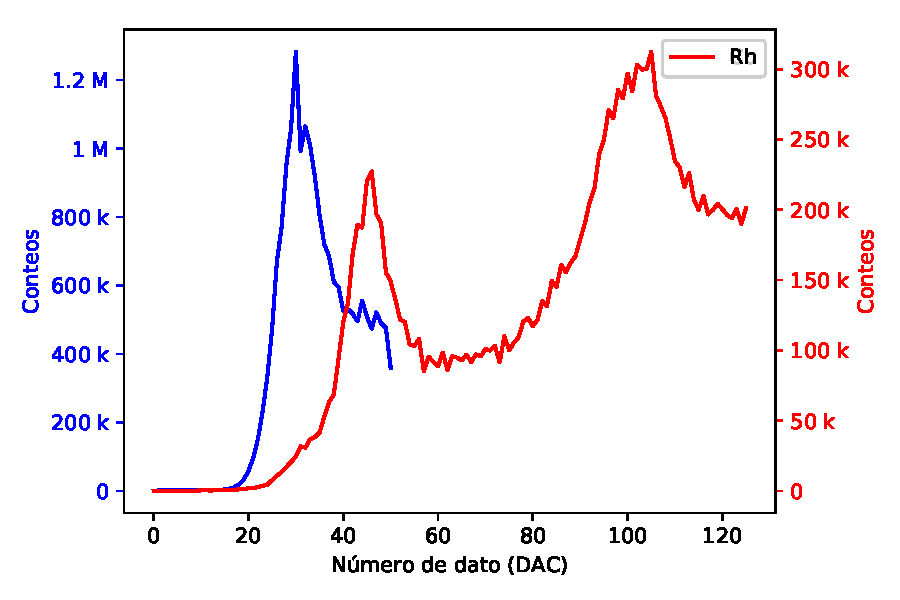
\includegraphics[width = \linewidth]{Figuras/CalibracionE.pdf}
	\end{figure}

	El número máximo de conteos escala con el voltaje del tubo.
	
	Cuando aumentan los voltajes aparecen más picos en el espectro.
	
	\begin{figure}[h]
		\centering
		\begin{tabular}{cc}
				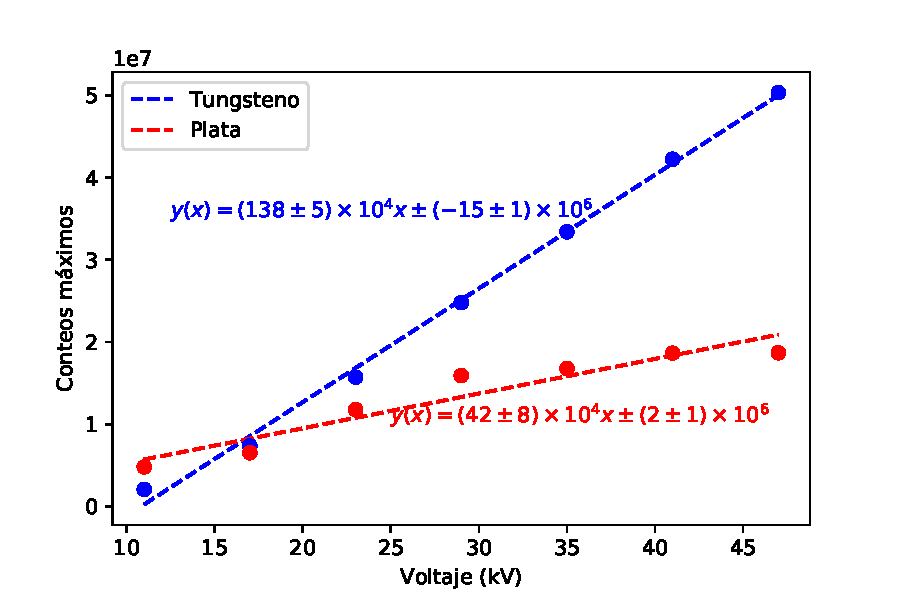
\includegraphics[width = 0.52\linewidth]{Figuras/Max_voltage.pdf}
				&
				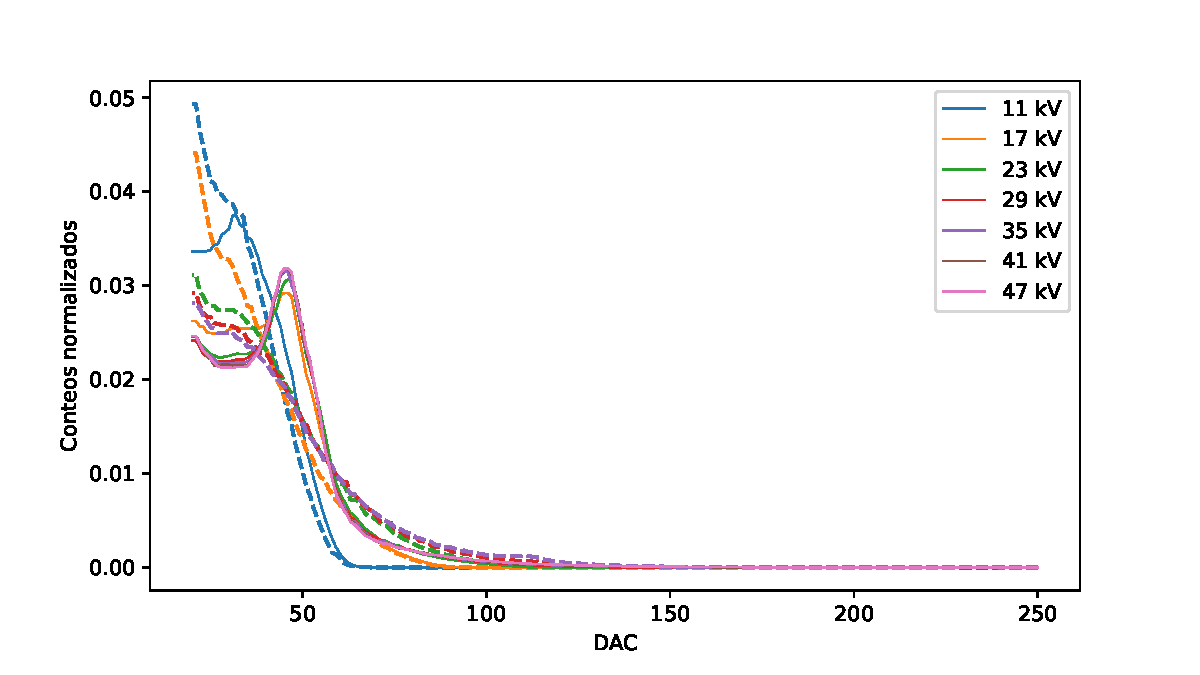
\includegraphics[width = 0.52\linewidth]{Figuras/Both_Normed.pdf}
		\end{tabular}
	\end{figure}
	
	La relación señal a ruido es baja a voltajes bajos (conteos de fuentes externas) y a voltajes altos (variaciones en las emisiones de la fuente).
	La relación de señal a ruido es más alta para el tungsteno, dada su mayor potencia de emisión.
	
	\begin{table}[h]
		\centering
		\begin{tabular}{cc}
			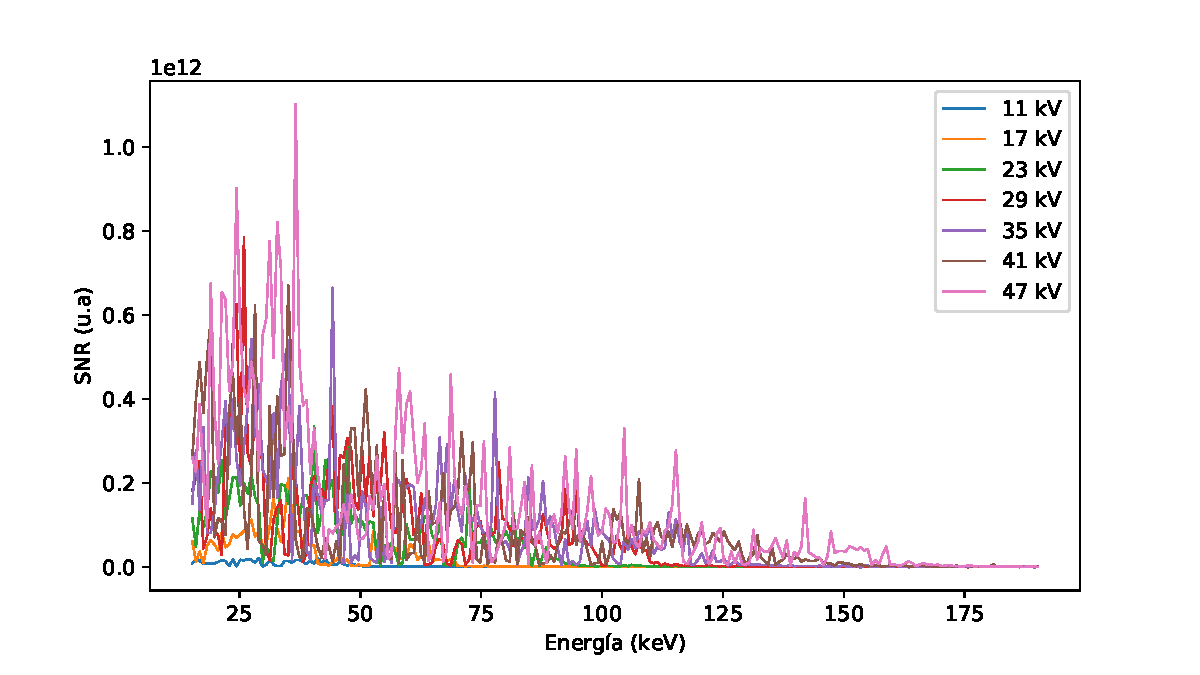
\includegraphics[width = 0.52\linewidth]{Figuras/wsnr.pdf}
			&
			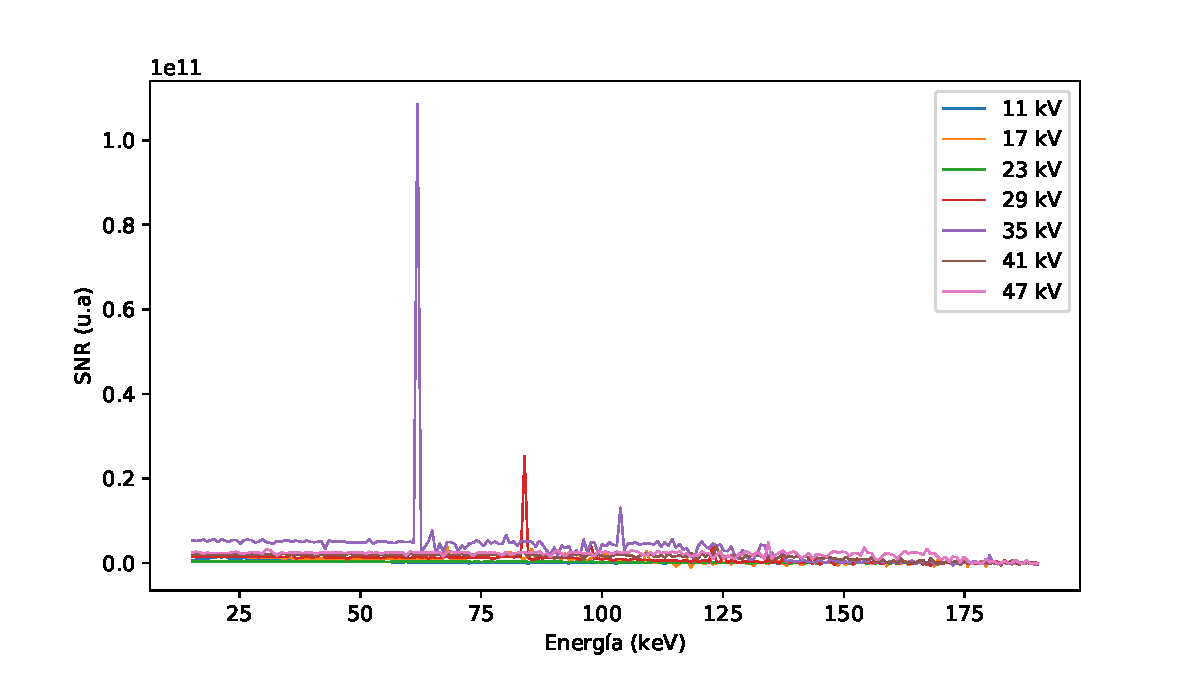
\includegraphics[width = 0.52\linewidth]{Figuras/agsnr.pdf}
		\end{tabular}
	\end{table}
	
	El contraste de las imágenes es más alto con la fuente de ánodo de plata.
	
	La fuente de ánodo de plata tiende a producir fotones más energéticos.
	
	\begin{figure}[h]
		\centering
		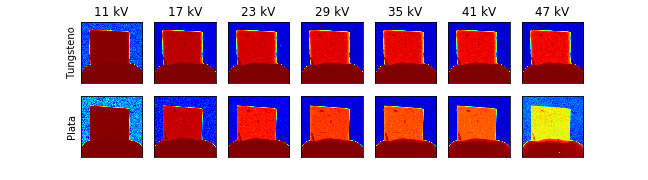
\includegraphics[width = \linewidth]{Figuras/Images.png}
	\end{figure}
	
	\begin{figure}[h]
		\centering
		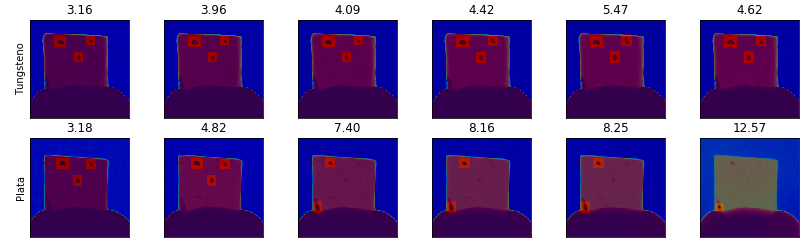
\includegraphics[width = \linewidth]{Figuras/ContrasteImages.png}
	\end{figure}
	
	La diferencia de contrastes crece con el voltaje del tubo.
	
	\begin{figure}[h]
		\centering
		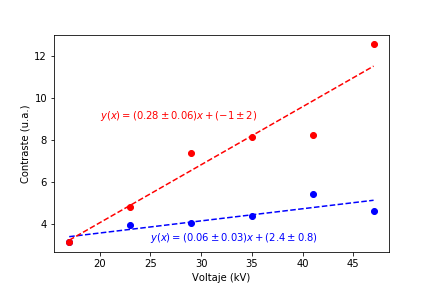
\includegraphics[width = \linewidth]{Figuras/Contraste.png}
	\end{figure}

\section{Conclusiones}

\begin{itemize}
	\item La función de relación de señal a ruido no es una función suave de la energía.
	\item La fuente de ánodo de plata es más eficiente a bajas energías.
	\item La fuente de ánodo de tungsteno es más eficiente a altas energías.
	\item El espectro observado mantiene su forma al superar ciertos valores de voltaje (23 kV en este caso).
\end{itemize}
%	 En general, se observó que la función de la relación de señal a ruido no es una función suave en la energía. Esto se debe en gran medida a los picos de emisión en los espectros de energía de los tubos de rayos X. Además se pueden concluir dos cosas, para voltajes de aceleración inferiores a 17 kV, la fuente de ánodo de plata es más brillante que la de tungsteno, este resultado posteriormente se invierte. Por otro lado la pendiente muestra que la fuente de tungsteno es tiene mayor eficiencia lumínica, dado que por cada voltio aplicado los conteos aumentan más del doble respecto a la fuente de plata.
%	 
%	 La morfología se mantiene constante para valores iguales o superiores a 23 kV, en ambas fuentes. Respecto a los errores experimentales se muestra que la incertidumbre para la fuente de tungsteno es completamente aleatoria, mientras que para el caso de la fuente de plata se tiene un error sistemático en las medidas.
	
\nocite{als2011elements,amtek,ballabriga2011medipix3,exper,koningsberger1988x,manualT,mendenhall2017high,mini,param,range,van2014scikit,xps}
\bibliographystyle{unsrt}
\tiny
\bibliography{bib}

\end{multicols}

\end{document}